\chapter{Ethernet LAN Switching: Part
2}\label{ethernet-lan-switching-part-2}

An ETHERNET FRAME looks like:

Ethernet Header --- DATA (Packet) --- Ethernet Trailer

\begin{figure}
\centering
\pandocbounded{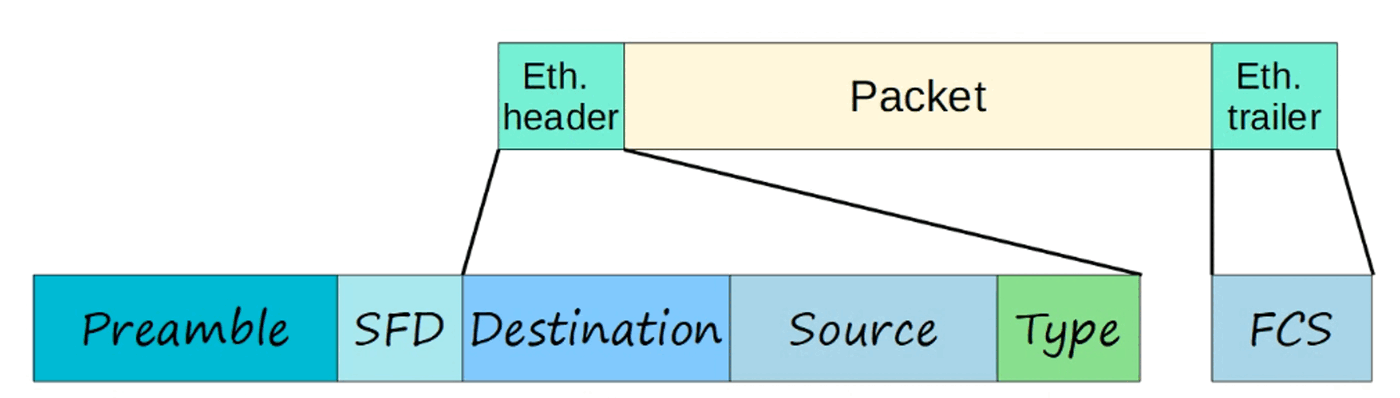
\includegraphics[keepaspectratio,alt={image}]{images/06-ethernet-lan-switching-part2/img-001.png}}
\end{figure}

The Ethernet Header contains 5 Fields:

Preamble -- SFD -- Destination -- Source -- Type/Length 7 bytes -- 1
byte -- 6 bytes -- 6 bytes -- 2 bytes

Ethernet Trailer contains 1 Field:

FCS (Frame Check Sequence) = 4 bytes

\begin{itemize}
\tightlist
\item
  The PREAMBLE + SFD is not usually considered part of the ETHERNET
  HEADER.
\end{itemize}

THEREFORE the size of the ETHERNET HEADER + TRAILER is 18 bytes

(6 + 6 + 2 + 4 bytes for the FRAME CHECK SEQUENCE)

The MINIMUM size for an ETHERNET FRAME (Header + Payload {[}PACKET{]} +
Trailer) is 64 BYTES.

64 BYTES - 18 BYTES (Header + Trailer size) = 46 BYTES

THEREFORE the MINIMUM DATA PAYLOAD (PACKET) size is 46 BYTES!

IF the PAYLOAD is LESS than 46 BYTES then PADDING BYTES are added
(padding bytes are a series of 0's) until it equals to 46 BYTES.

When a PC wants to send a packet to a destination, with a known IP
address but an unknown MAC address, it first needs to send an ARP
Request to learn that destination's MAC address.

\begin{figure}
\centering
\pandocbounded{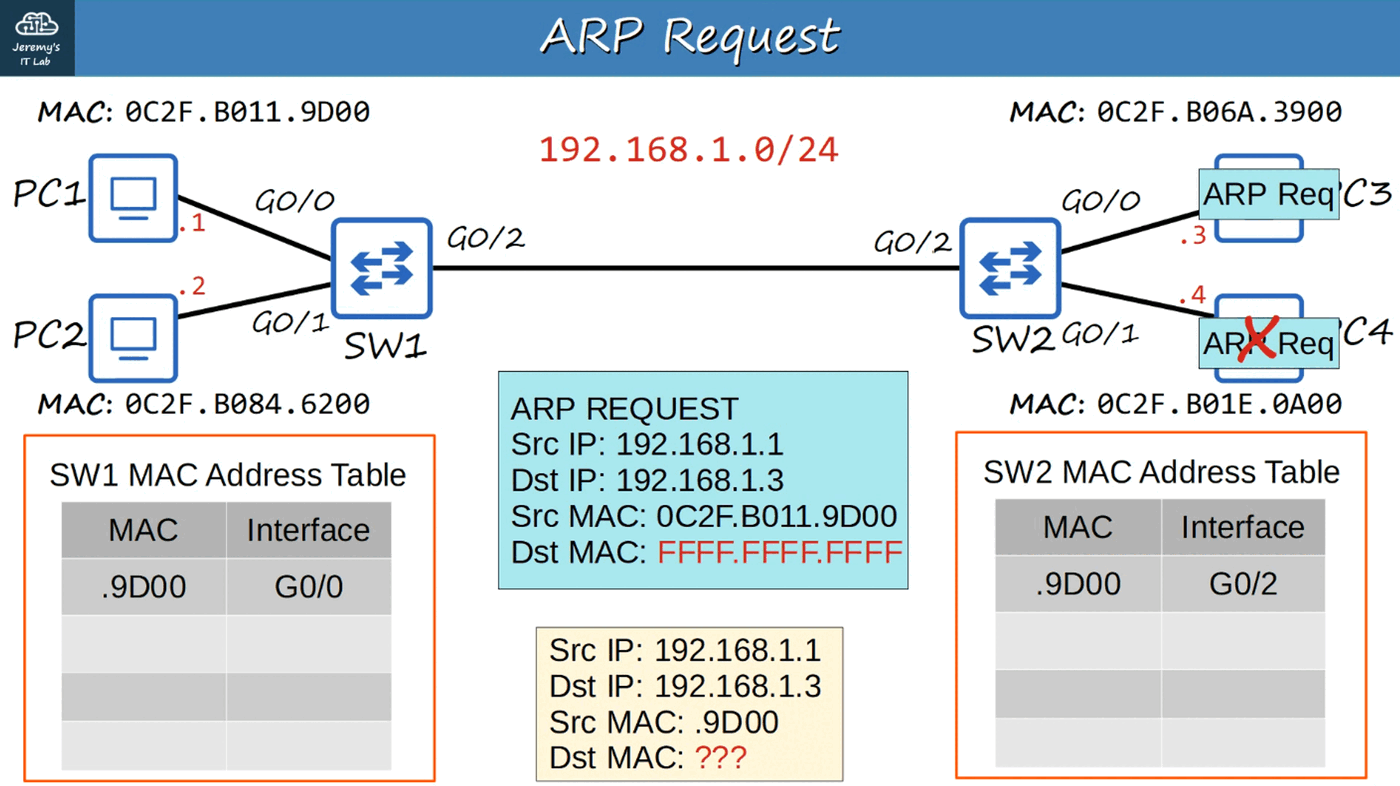
\includegraphics[keepaspectratio,alt={image}]{images/06-ethernet-lan-switching-part2/img-002.png}}
\end{figure}

\begin{itemize}
\tightlist
\item
  ARP stands for `Address Resolution Protocol'.
\item
  It is used to discover the Layer 2 address (MAC address) of a known
  Layer 3 address (IP address)
\item
  Consists of two messages:

  \begin{itemize}
  \tightlist
  \item
    ARP REQUEST (Source message)
  \item
    ARP REPLY (Destination message)
  \end{itemize}
\item
  ARP REQUEST is BROADCAST = sent to all hosts on network, except the
  one it received the request from.
\end{itemize}

An ARP REQUEST frame has:

\begin{itemize}
\tightlist
\item
  Source IP Address
\item
  Destination IP Address
\item
  Source MAC address
\item
  BROADCAST MAC Address - FFFF.FFFF.FFFF
\end{itemize}

An ARP REPLY frame has:

\begin{itemize}
\tightlist
\item
  Source IP Address
\item
  Destination IP Address
\item
  Source MAC address
\item
  Destination MAC Address
\end{itemize}

ARP REPLY is a known UNICAST frame = Sent only to the host that sent the
ARP REQUEST.

\begin{figure}
\centering
\pandocbounded{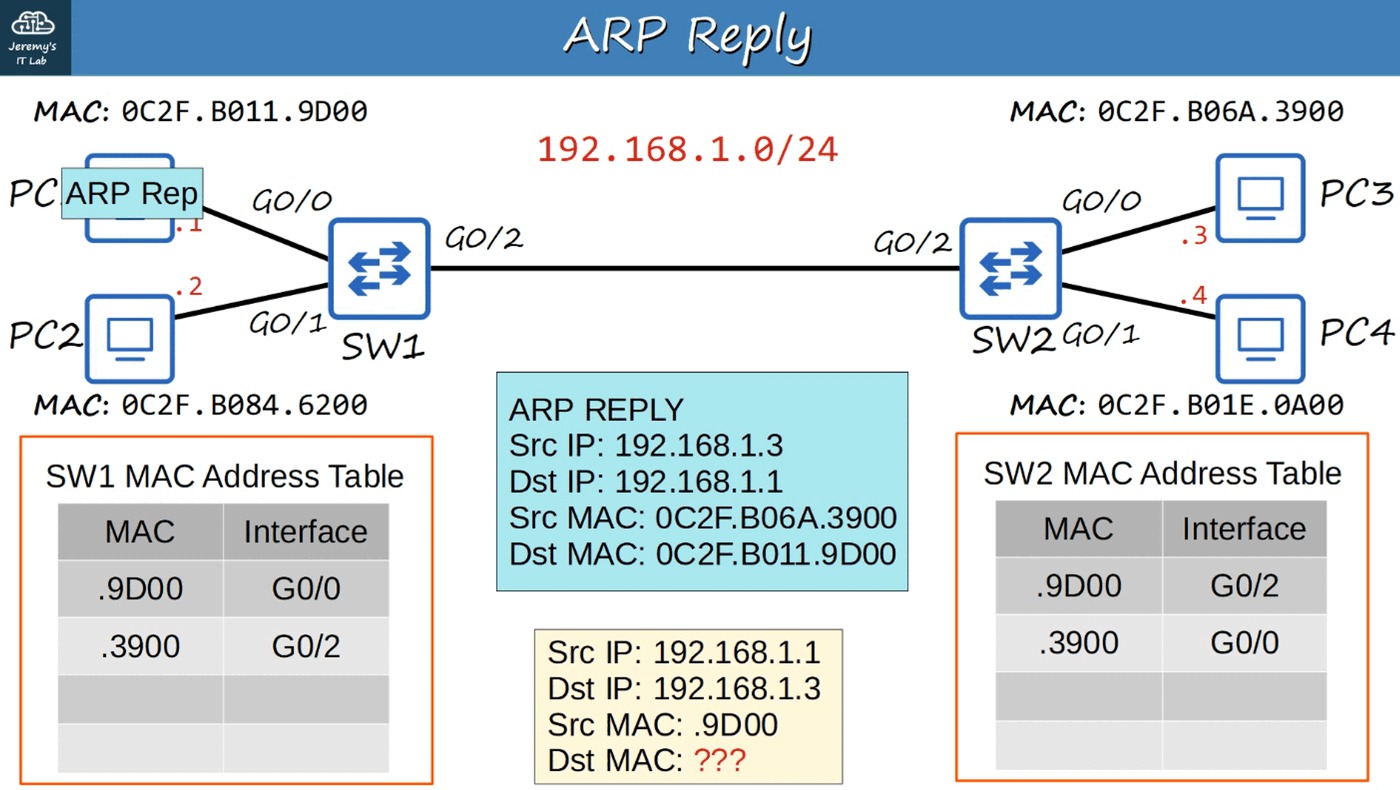
\includegraphics[keepaspectratio,alt={image}]{images/06-ethernet-lan-switching-part2/img-003.png}}
\end{figure}

\section{Ping}\label{ping}

\begin{itemize}
\tightlist
\item
  A network utility that is used to test reachability
\item
  Measures round-trip time
\item
  Uses two messages:

  \begin{itemize}
  \tightlist
  \item
    ICMP Echo REQUEST
  \item
    ICMP Echo REPLY
  \end{itemize}
\item
  Is UNICAST
\item
  Command to use ping:

  \begin{itemize}
  \tightlist
  \item
    ping \textless ip-address\textgreater{}
  \end{itemize}
\end{itemize}

By Default, a CISCO IOS sends 5 ICMP requests/replies (Default size is
100-bytes)

\begin{itemize}
\tightlist
\item
  A period (.) is a failed ping
\item
  An exclamation mark (!) is a successful ping
\end{itemize}

USEFUL CISCO IOS COMMANDS (from Privileged EXEC mode)

PC1\# show arp // shows hosts ARP table

\begin{figure}
\centering
\pandocbounded{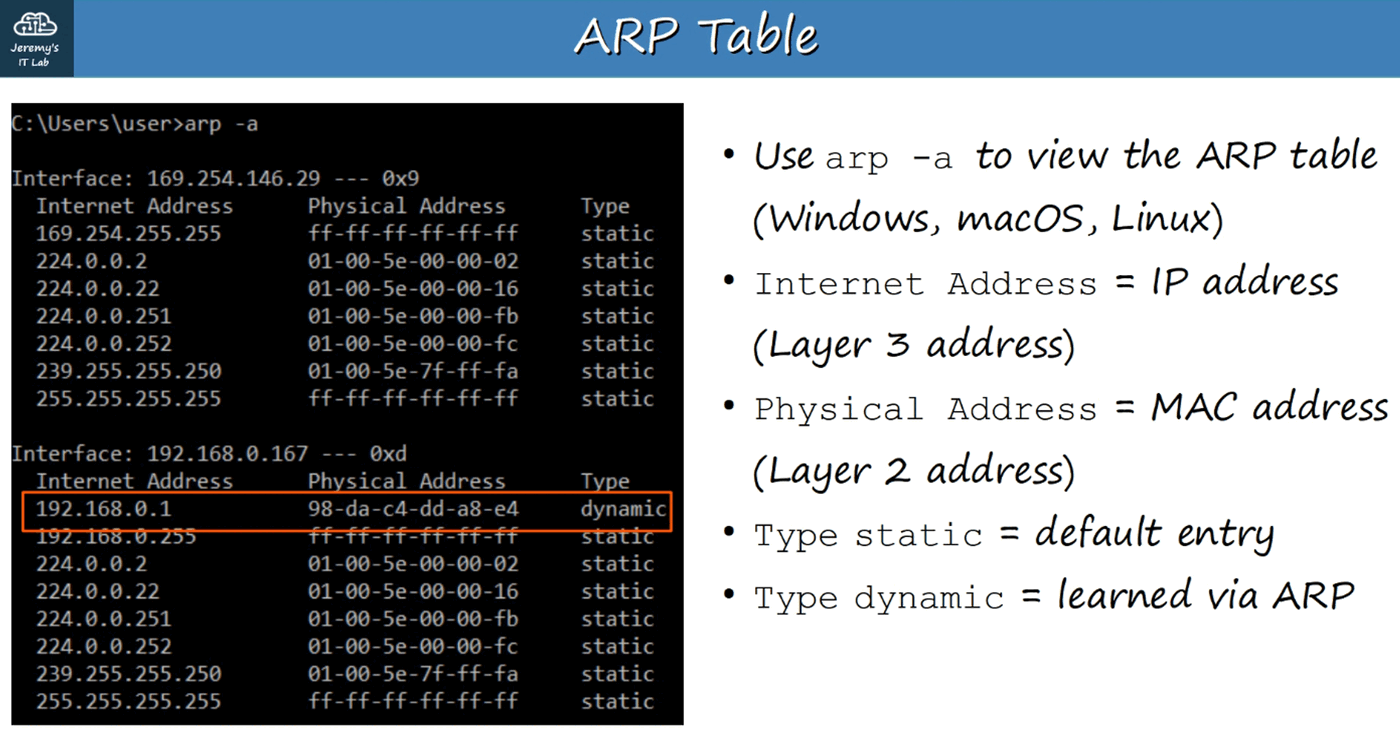
\includegraphics[keepaspectratio,alt={image}]{images/06-ethernet-lan-switching-part2/img-004.png}}
\end{figure}

SW1\#show mac address-table // show the switches MAC table

\begin{figure}
\centering
\pandocbounded{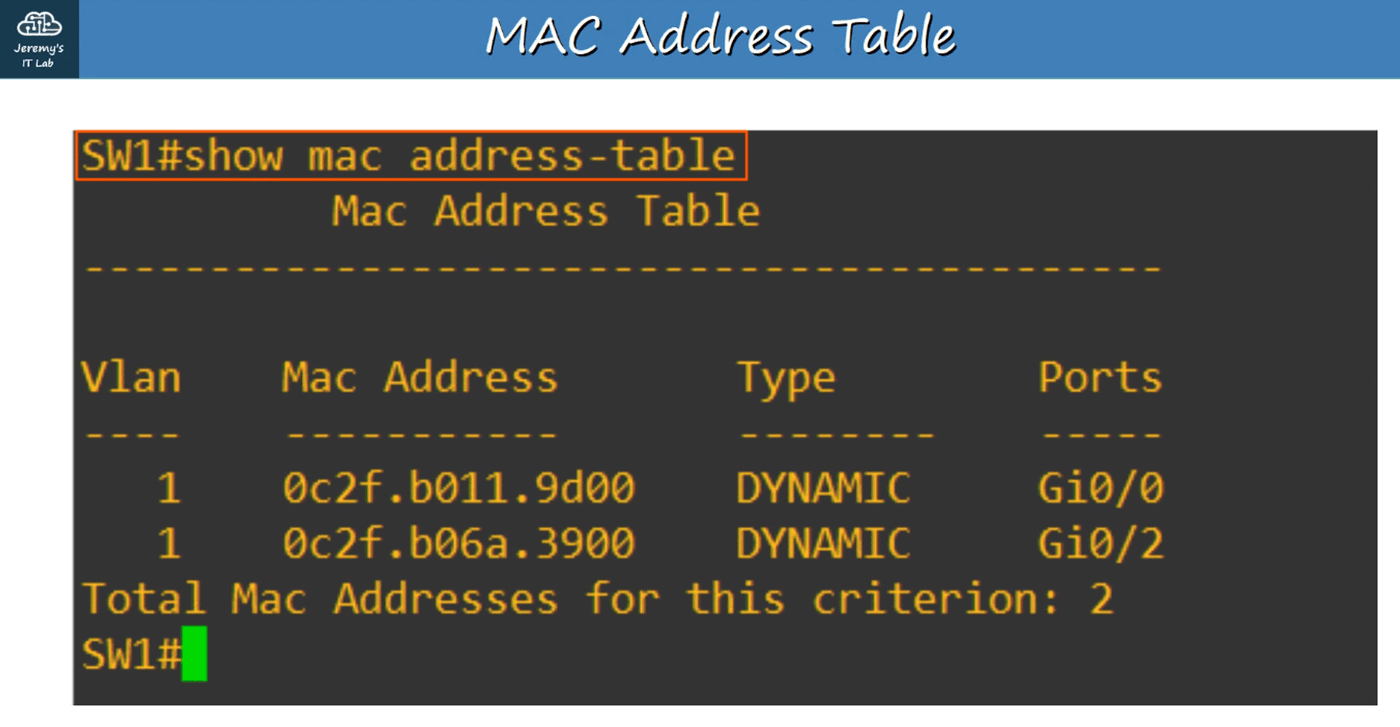
\includegraphics[keepaspectratio,alt={image}]{images/06-ethernet-lan-switching-part2/img-005.png}}
\end{figure}

Will show:

Vlan --- MAC Address --- Type --- Ports(interfaces)

(Vlan = Virtual Local Area Network)

\begin{figure}
\centering
\pandocbounded{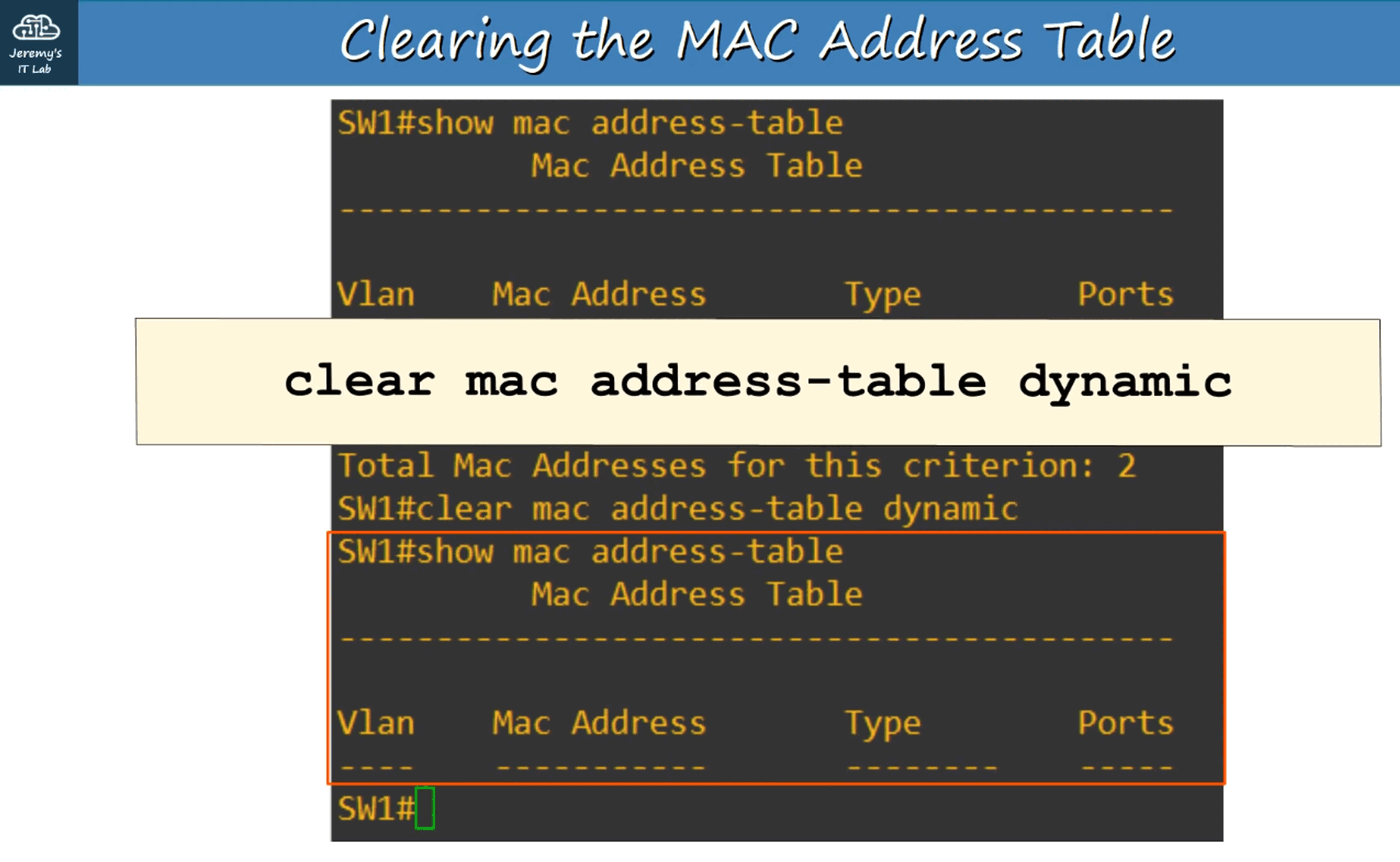
\includegraphics[keepaspectratio,alt={image}]{images/06-ethernet-lan-switching-part2/img-006.png}}
\end{figure}

SW1\# clear mac address-table dynamic \textless optional MAC
address\textgreater{}

// clears the entire switches MAC table. // IF the optional MAC address
is used, it will clear the SPECFIC MAC address.

SW1 \#clear mac address-table dynamic interface \textless optional
Interface\textgreater{}

// clears the MAC table entry of the Switch by it's \textbf{INTERFACE
n}ame.
